\chapter{Kleurgebaseerde similariteitsmaten}

In dit hoofdstuk construeren we enkele similariteitsmaten die beelden 
vergelijken op basis van de kleuren die er in voorkomen. Het universum wordt
in dit geval dus gevormd door de kleuren in plaats van de beeldpunten. Vermits kleur \'e\'en 
van de meest gebruikte kenmerken is bij CBIR \cite{rui:image_retr}, mogen we 
verwachten dat die \emph{kleurgebaseerde} aanpak effici\"ente 
similariteitsmaten zal opleveren. 

Een histogram van een kleurbeeld is een voorstelling van de frequentieverdeling 
van de verschillende kleuren. De waarde van het histogram voor een kleurbeeld 
$A$ in de kleur $c$ is dus gelijk aan het totaal aantal pixels in het beeld met 
kleur $c$. We noteren dit met $h_A(c)$: $$ h_A(c) = \sum_{x \in X} \delta (c - 
A(x)) $$ waarbij $\delta$ de Diracfuntie is en $X$ het universum der beelpunten 
voorstelt.


\section{Pseudo-vage histogrammen}

Door de waarden van een histogram te normaliseren, kunnen we het omzetten naar 
een vaagverzameling in het universum der kleuren $C$. Dit houdt in dat we elke 
waarde van het histogram delen door het maximaal aantal pixels met dezelfde 
kleur. We hebben dus de volgende uitdrukking voor de lidmaatschapsgraad van de 
kleur $c$ in de vaagverzameling $\mathit{PFh}_A$ geassocieerd met het histogram 
van beeld $A$: $$
\mathit{PFh}_A(c) = \frac{\displaystyle h_A(c)}{\displaystyle \max_{c \in C}(h_A(c))}
$$ De kleur die het meest voorkomt heeft dus lidmaatschapsgraad $1$. Alle 
andere kleuren hebben kleinere lidmaatschapsgraden.

%Voor een RGB-beeld gebruikt men typisch 8 bits per kleurcomponent. Dit geeft een totaal van
%24 bits per kleur, zodat men dus $2^{24}=2^4 \cdot 2^{20}=16 \cdot 2^{20} \approx 16 \cdot 10^6$
%kleuren kan voorstellen. Een genormaliseerd histogram bestaat dan dus uit 16 miljoen waarden.
%Similariteitsmaten op basis van dergelijke histogrammen zouden dus veel te veel rekentijd vragen.

Om de rekentijd te beperken, maken we gebruik van kleurkwantisatie. 
De karakteristieke afbeelding van de vaagverzameling $\mathit{BPFh}_A$, die
correspondeert met het in $N$ bins onderverdeelde histogram van beeld $A$, wordt dan als volgt
gedefinieerd:  
$$
\begin{array}{lrcl}
\mathit{BPFh}_A: 	& \{1,2,\ldots,N\} 	& \to 		& [0,1] \\[5pt]
		& n						& \mapsto	& \displaystyle\sum_{c \in C} \delta (n -  bin(c)),
\quad\forall n \in \{1,2,\ldots,N\}
\end{array}
$$
Hierbij is $bin$ de $C - \{1,2,\ldots,N\}$ afbeelding uit \ref{sectie:kleurkwantisatie}, die met 
elke kleur het nummer van de corresponderende bin associeert. 


\section{Vaaghistogrammen}

Naast de bovenstaande vage interpretatie van het klassieke kleurhistogram, 
beschouwen we ook nog een gelijkaardige kleurbeschrijving die we op een 
``volledig vage'' manier opbouwen. Bij dit \emph{vaaghistogram} maken we 
gebruik van het (niet genormaliseerde) L*a*b* kleurmodel en beschouwen we een 
vaagverzameling voor elke kleur. De lidmaatschapsgraad van een kleur $c'$ in de 
vaagverzameling $FC_c$, die correspondeert met kleur $c$, defini\"eren we als 
volgt \cite{vertan:embedding_fuzzy_logic_in_cbir,vertan:fuzzy_histograms}: $$
\begin{array}{rcll}
FC_c(c') & = & 1 & \textrm{als } d(c,c') \leq 2.3 \\ & = & \exp \left( - 
\frac{\left((d(c,c') / 2.3) - 1\right)^2}{2 \cdot \lambda^2} \right) & 
\textrm{anders}
\end{array}
$$ met $d$ de Euclidische afstand en $\lambda$ een vrij te kiezen parameter, 
die we in deze scriptie voor de eenvoud steeds gelijk aan $1$ zullen kiezen. In 
het geval van L*a*b* komt de afstand $2.3$ namelijk overeen met de zogenaamde 
\emph{just noticeable difference} (JND) \cite{sharma:digital_color_imaging}. 
Kleuren waarvan de onderlinge afstand kleiner dan of gelijk aan deze JND is, 
kunnen door de mens niet onderscheiden worden.

Het eigenlijk vaaghistogram $Fh_A$, voor een kleurbeeld $A$, defini\"eren we 
dan als de unie van alle kleuren die voorkomen in $A$: $$ Fh_A = 
\displaystyle\bigcup_{c \in C_A} FC_c
%\begin{array}{lrcl}
%Fh_A: 	& C_A 	& \to 		& [0,1] \\[5pt]
%		& c					& \mapsto	& \displaystyle\bigcup_{c \in C_A} FC_c,
%\quad\forall c \in C_A
%\end{array}
$$ waarbij de verzameling $C_A$ bestaat uit de in $A$ voorkomende kleuren. Alle 
kleuren die (niet te onderscheiden zijn van kleuren die) voorkomen in het beeld 
hebben dus lidmaatschapsgraad $1$. De overige kleuren hebben kleinere 
lidmaatschapsgraden.


\section{Experimentele observaties}

%Het I1I2i3-model van Ohta is een goede benadering van de Karhunen-Loeve transformatie 
%voor het decorreleren van de RGB-componenten, waardoor het zeer geschikt is 
%voor beeldverwerking.

\begin{figure}[tbp]
\begin{center}
\includegraphics[width=\textwidth]{/home/klbostee/Workspace/Thesis/plots/histgeb1_gggrs_en_cputimes_filled.eps} 
\includegraphics[width=\textwidth]{/home/klbostee/Workspace/Thesis/plots/histgeb2_gggrs_en_cputimes_filled.eps}
\caption{\label{fig:histgeb_gggrs_en_cputimes}De GGGR-waarde en de gebruikte rekentijd in ms voor elk van de similariteitsmaten op basis van histrogrammen.}
\end{center}
\end{figure}

\begin{figure}[tbp]
\begin{center}
\begin{tabular}{m{11cm} | m{3cm} |}
\textbf{Eerste tien resultaten:} & \textbf{GGR:} \\
\vspace{4pt}
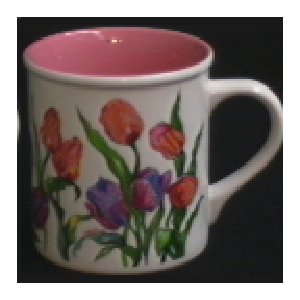
\includegraphics[width=1cm]{coil/beeld-6.eps} 
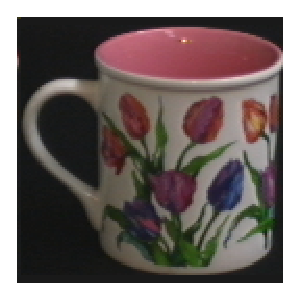
\includegraphics[width=1cm]{coil/beeld-7.eps} 
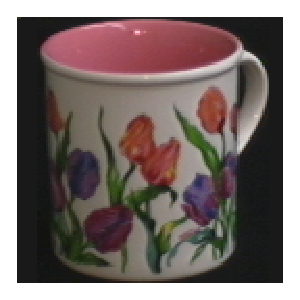
\includegraphics[width=1cm]{coil/beeld-9.eps} 
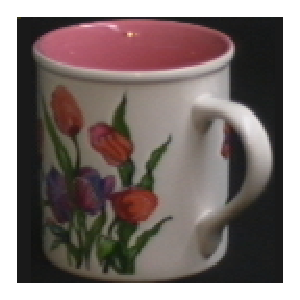
\includegraphics[width=1cm]{coil/beeld-10.eps} 
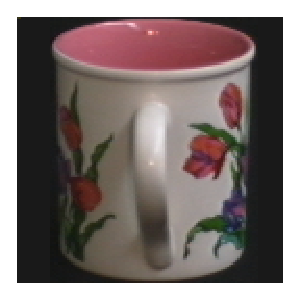
\includegraphics[width=1cm]{coil/beeld-11.eps} 
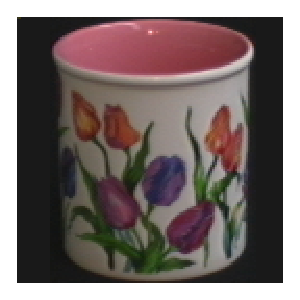
\includegraphics[width=1cm]{coil/beeld-8.eps} 
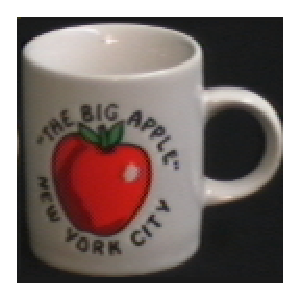
\includegraphics[width=1cm]{coil/beeld-36.eps} 
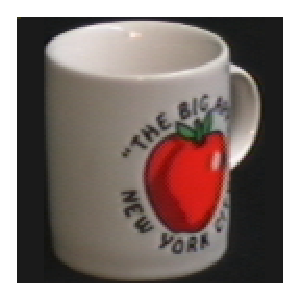
\includegraphics[width=1cm]{coil/beeld-39.eps} 
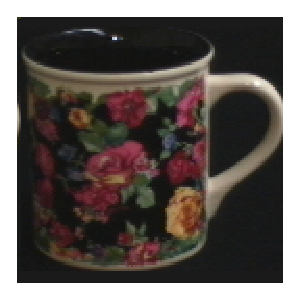
\includegraphics[width=1cm]{coil/beeld-60.eps} 
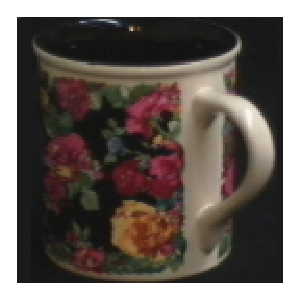
\includegraphics[width=1cm]{coil/beeld-64.eps} & {\scriptsize 0.0} \\ 

\includegraphics[width=1cm]{coil/beeld-18.eps} 
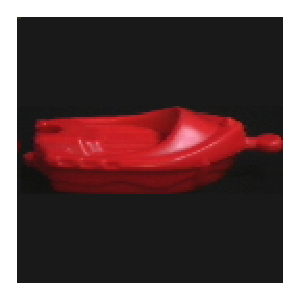
\includegraphics[width=1cm]{coil/beeld-19.eps} 
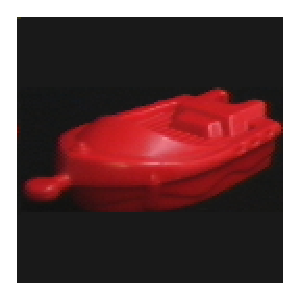
\includegraphics[width=1cm]{coil/beeld-21.eps} 
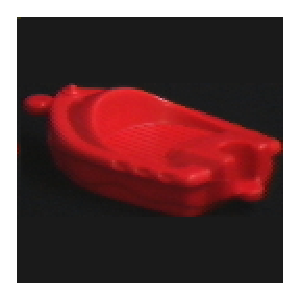
\includegraphics[width=1cm]{coil/beeld-22.eps} 
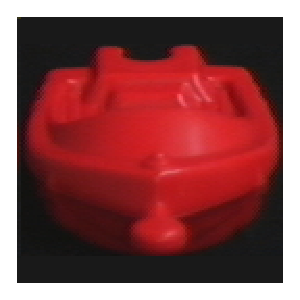
\includegraphics[width=1cm]{coil/beeld-20.eps} 
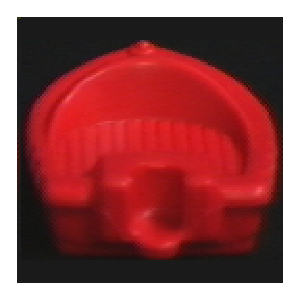
\includegraphics[width=1cm]{coil/beeld-23.eps} 
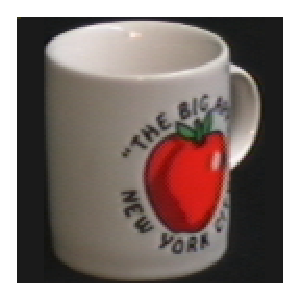
\includegraphics[width=1cm]{coil/beeld-39.eps} 
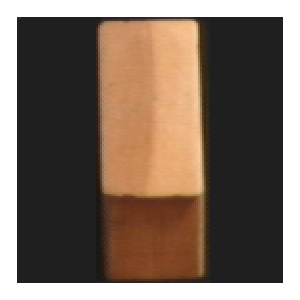
\includegraphics[width=1cm]{coil/beeld-44.eps} 
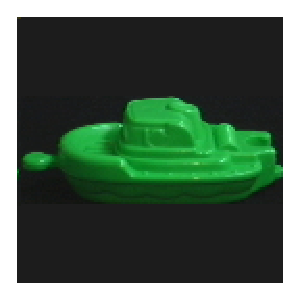
\includegraphics[width=1cm]{coil/beeld-54.eps} 
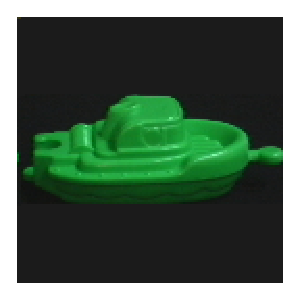
\includegraphics[width=1cm]{coil/beeld-55.eps} & {\scriptsize 0.0} \\ 
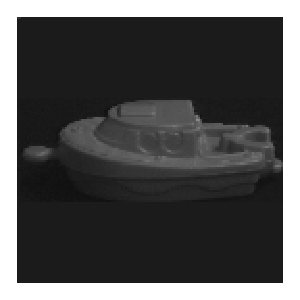
\includegraphics[width=1cm]{coil/beeld-24.eps} 
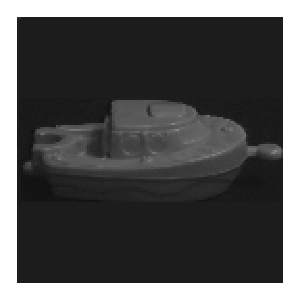
\includegraphics[width=1cm]{coil/beeld-25.eps} 
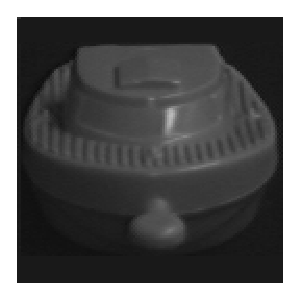
\includegraphics[width=1cm]{coil/beeld-28.eps} 
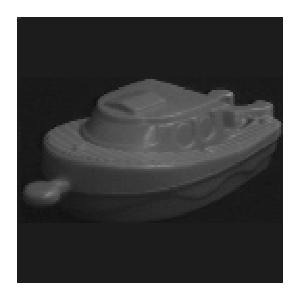
\includegraphics[width=1cm]{coil/beeld-27.eps} 
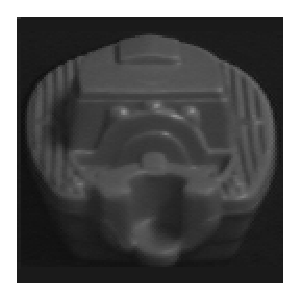
\includegraphics[width=1cm]{coil/beeld-26.eps} 
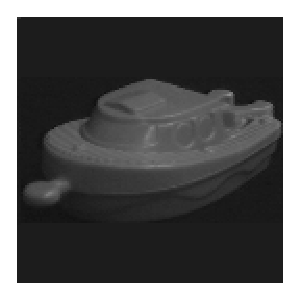
\includegraphics[width=1cm]{coil/beeld-29.eps} 
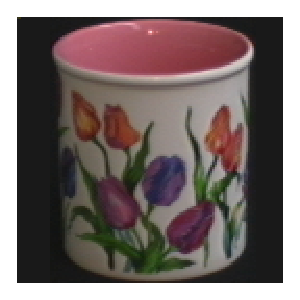
\includegraphics[width=1cm]{coil/beeld-8.eps} 
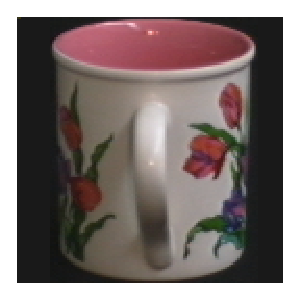
\includegraphics[width=1cm]{coil/beeld-11.eps} 
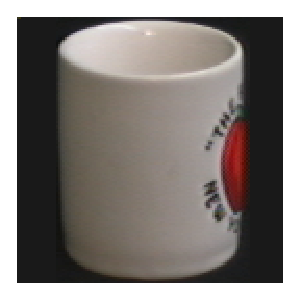
\includegraphics[width=1cm]{coil/beeld-38.eps} 
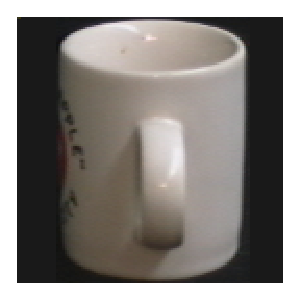
\includegraphics[width=1cm]{coil/beeld-41.eps} & {\scriptsize 0.0} \\ 
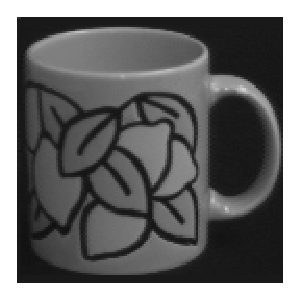
\includegraphics[width=1cm]{coil/beeld-48.eps} 
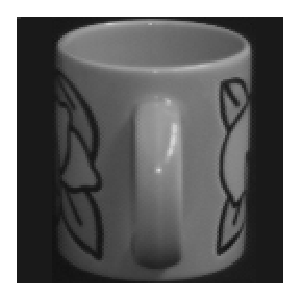
\includegraphics[width=1cm]{coil/beeld-50.eps} 
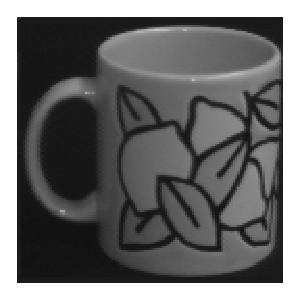
\includegraphics[width=1cm]{coil/beeld-49.eps} 
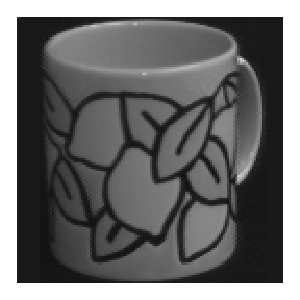
\includegraphics[width=1cm]{coil/beeld-51.eps} 
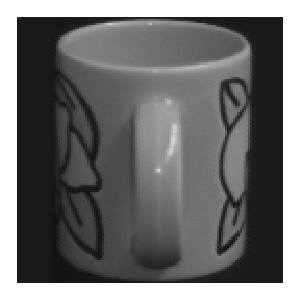
\includegraphics[width=1cm]{coil/beeld-53.eps} 
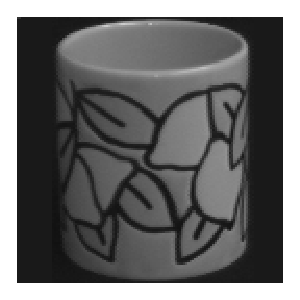
\includegraphics[width=1cm]{coil/beeld-52.eps} 
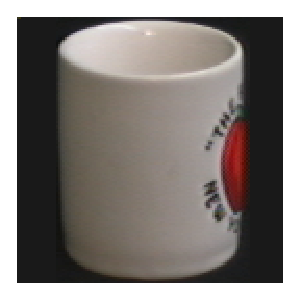
\includegraphics[width=1cm]{coil/beeld-38.eps} 
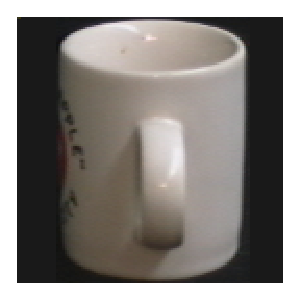
\includegraphics[width=1cm]{coil/beeld-41.eps} 
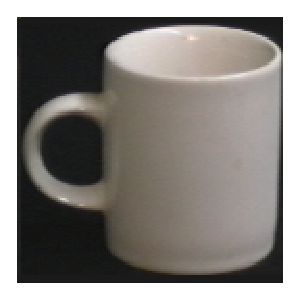
\includegraphics[width=1cm]{coil/beeld-37.eps} 
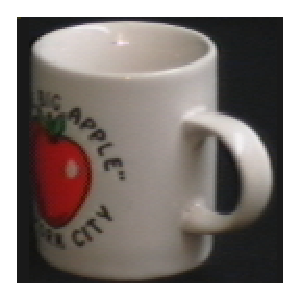
\includegraphics[width=1cm]{coil/beeld-40.eps} & {\scriptsize 0.0} \\ 
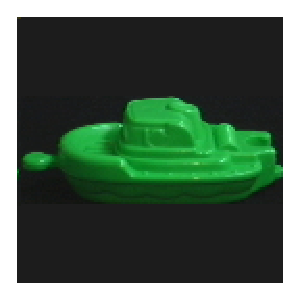
\includegraphics[width=1cm]{coil/beeld-54.eps} 
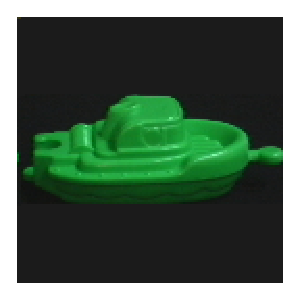
\includegraphics[width=1cm]{coil/beeld-55.eps} 
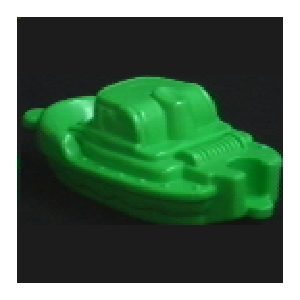
\includegraphics[width=1cm]{coil/beeld-58.eps} 
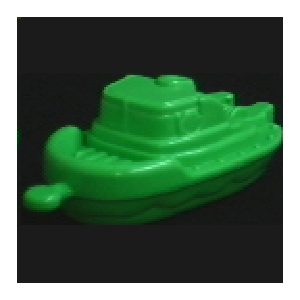
\includegraphics[width=1cm]{coil/beeld-57.eps} 
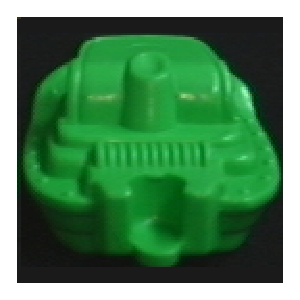
\includegraphics[width=1cm]{coil/beeld-59.eps} 
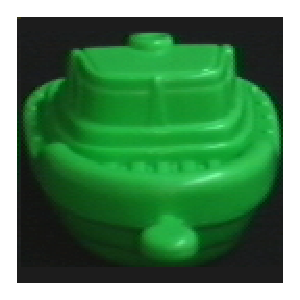
\includegraphics[width=1cm]{coil/beeld-56.eps} 
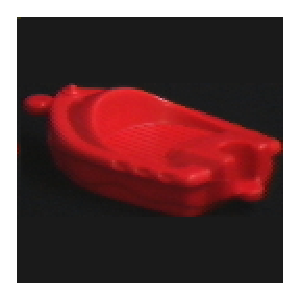
\includegraphics[width=1cm]{coil/beeld-22.eps} 
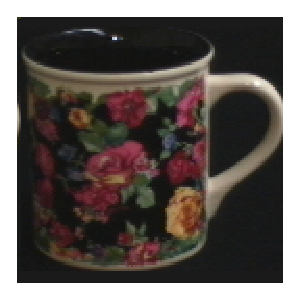
\includegraphics[width=1cm]{coil/beeld-60.eps} 
\includegraphics[width=1cm]{coil/beeld-21.eps} 
\includegraphics[width=1cm]{coil/beeld-63.eps} & {\scriptsize 0.0} \\ 
\includegraphics[width=1cm]{coil/beeld-60.eps} 
\includegraphics[width=1cm]{coil/beeld-61.eps} 
\includegraphics[width=1cm]{coil/beeld-64.eps} 
\includegraphics[width=1cm]{coil/beeld-63.eps} 
\includegraphics[width=1cm]{coil/beeld-65.eps} 
\includegraphics[width=1cm]{coil/beeld-62.eps} 
\includegraphics[width=1cm]{coil/beeld-7.eps} 
\includegraphics[width=1cm]{coil/beeld-9.eps} 
\includegraphics[width=1cm]{coil/beeld-10.eps} 
\includegraphics[width=1cm]{coil/beeld-8.eps} & {\scriptsize 0.0} \\ 
\includegraphics[width=1cm]{coil/beeld-12.eps} 
\includegraphics[width=1cm]{coil/beeld-13.eps} 
\includegraphics[width=1cm]{coil/beeld-16.eps} 
\includegraphics[width=1cm]{coil/beeld-15.eps} 
\includegraphics[width=1cm]{coil/beeld-14.eps} 
\includegraphics[width=1cm]{coil/beeld-62.eps} 
\includegraphics[width=1cm]{coil/beeld-17.eps} 
\includegraphics[width=1cm]{coil/beeld-65.eps} 
\includegraphics[width=1cm]{coil/beeld-21.eps} 
\includegraphics[width=1cm]{coil/beeld-57.eps} & {\scriptsize 
0.002380952380952381} \\ \includegraphics[width=1cm]{coil/beeld-30.eps} 
\includegraphics[width=1cm]{coil/beeld-31.eps} 
\includegraphics[width=1cm]{coil/beeld-34.eps} 
\includegraphics[width=1cm]{coil/beeld-33.eps} 
\includegraphics[width=1cm]{coil/beeld-32.eps} 
\includegraphics[width=1cm]{coil/beeld-61.eps} 
\includegraphics[width=1cm]{coil/beeld-35.eps} 
\includegraphics[width=1cm]{coil/beeld-64.eps} 
\includegraphics[width=1cm]{coil/beeld-60.eps} 
\includegraphics[width=1cm]{coil/beeld-40.eps} & {\scriptsize 
0.002380952380952381} \\ \includegraphics[width=1cm]{coil/beeld-36.eps} 
\includegraphics[width=1cm]{coil/beeld-40.eps} 
\includegraphics[width=1cm]{coil/beeld-37.eps} 
\includegraphics[width=1cm]{coil/beeld-39.eps} 
\includegraphics[width=1cm]{coil/beeld-10.eps} 
\includegraphics[width=1cm]{coil/beeld-9.eps} 
\includegraphics[width=1cm]{coil/beeld-7.eps} 
\includegraphics[width=1cm]{coil/beeld-38.eps} 
\includegraphics[width=1cm]{coil/beeld-41.eps} 
\includegraphics[width=1cm]{coil/beeld-6.eps} & {\scriptsize 
0.014285714285714285} \\ \includegraphics[width=1cm]{coil/beeld-0.eps} 
\includegraphics[width=1cm]{coil/beeld-1.eps} 
\includegraphics[width=1cm]{coil/beeld-42.eps} 
\includegraphics[width=1cm]{coil/beeld-4.eps} 
\includegraphics[width=1cm]{coil/beeld-43.eps} 
\includegraphics[width=1cm]{coil/beeld-3.eps} 
\includegraphics[width=1cm]{coil/beeld-45.eps} 
\includegraphics[width=1cm]{coil/beeld-46.eps} 
\includegraphics[width=1cm]{coil/beeld-37.eps} 
\includegraphics[width=1cm]{coil/beeld-62.eps} & {\scriptsize 
0.11666666666666667} \\ \includegraphics[width=1cm]{coil/beeld-42.eps} 
\includegraphics[width=1cm]{coil/beeld-0.eps} 
\includegraphics[width=1cm]{coil/beeld-1.eps} 
\includegraphics[width=1cm]{coil/beeld-4.eps} 
\includegraphics[width=1cm]{coil/beeld-43.eps} 
\includegraphics[width=1cm]{coil/beeld-3.eps} 
\includegraphics[width=1cm]{coil/beeld-46.eps} 
\includegraphics[width=1cm]{coil/beeld-45.eps} 
\includegraphics[width=1cm]{coil/beeld-37.eps} 
\includegraphics[width=1cm]{coil/beeld-62.eps} & {\scriptsize 
0.2357142857142857}
\end{tabular}
\caption{\label{fig:results_i1i2i3_histgeb}De GGR-waarde en de eerste tien resultaten voor elk voorbeeld bij de beste similariteitsmaat op basis van het I1I2I3-histogram.}
\end{center}
\end{figure}

\begin{figure}[tbp]
\begin{center}
\begin{tabular}{m{11cm} | m{3cm} |}
\textbf{Eerste tien resultaten:} & \textbf{GGR:} \\
\vspace{4pt}
\includegraphics[width=1cm]{coil/beeld-12.eps} 
\includegraphics[width=1cm]{coil/beeld-13.eps} 
\includegraphics[width=1cm]{coil/beeld-15.eps} 
\includegraphics[width=1cm]{coil/beeld-16.eps} 
\includegraphics[width=1cm]{coil/beeld-17.eps} 
\includegraphics[width=1cm]{coil/beeld-14.eps} 
\includegraphics[width=1cm]{coil/beeld-44.eps} 
\includegraphics[width=1cm]{coil/beeld-47.eps} 
\includegraphics[width=1cm]{coil/beeld-5.eps} 
\includegraphics[width=1cm]{coil/beeld-2.eps} & {\scriptsize 0.0} \\ 
\includegraphics[width=1cm]{coil/beeld-6.eps} 
\includegraphics[width=1cm]{coil/beeld-7.eps} 
\includegraphics[width=1cm]{coil/beeld-8.eps} 
\includegraphics[width=1cm]{coil/beeld-9.eps} 
\includegraphics[width=1cm]{coil/beeld-11.eps} 
\includegraphics[width=1cm]{coil/beeld-10.eps} 
\includegraphics[width=1cm]{coil/beeld-65.eps} 
\includegraphics[width=1cm]{coil/beeld-41.eps} 
\includegraphics[width=1cm]{coil/beeld-64.eps} 
\includegraphics[width=1cm]{coil/beeld-36.eps} & {\scriptsize 0.0} \\ 
\includegraphics[width=1cm]{coil/beeld-18.eps} 
\includegraphics[width=1cm]{coil/beeld-19.eps} 
\includegraphics[width=1cm]{coil/beeld-21.eps} 
\includegraphics[width=1cm]{coil/beeld-22.eps} 
\includegraphics[width=1cm]{coil/beeld-20.eps} 
\includegraphics[width=1cm]{coil/beeld-23.eps} 
\includegraphics[width=1cm]{coil/beeld-32.eps} 
\includegraphics[width=1cm]{coil/beeld-36.eps} 
\includegraphics[width=1cm]{coil/beeld-33.eps} 
\includegraphics[width=1cm]{coil/beeld-39.eps} & {\scriptsize 0.0} \\ 
\includegraphics[width=1cm]{coil/beeld-24.eps} 
\includegraphics[width=1cm]{coil/beeld-25.eps} 
\includegraphics[width=1cm]{coil/beeld-28.eps} 
\includegraphics[width=1cm]{coil/beeld-27.eps} 
\includegraphics[width=1cm]{coil/beeld-26.eps} 
\includegraphics[width=1cm]{coil/beeld-29.eps} 
\includegraphics[width=1cm]{coil/beeld-39.eps} 
\includegraphics[width=1cm]{coil/beeld-38.eps} 
\includegraphics[width=1cm]{coil/beeld-7.eps} 
\includegraphics[width=1cm]{coil/beeld-6.eps} & {\scriptsize 0.0} \\ 
\includegraphics[width=1cm]{coil/beeld-30.eps} 
\includegraphics[width=1cm]{coil/beeld-32.eps} 
\includegraphics[width=1cm]{coil/beeld-31.eps} 
\includegraphics[width=1cm]{coil/beeld-33.eps} 
\includegraphics[width=1cm]{coil/beeld-34.eps} 
\includegraphics[width=1cm]{coil/beeld-35.eps} 
\includegraphics[width=1cm]{coil/beeld-60.eps} 
\includegraphics[width=1cm]{coil/beeld-63.eps} 
\includegraphics[width=1cm]{coil/beeld-61.eps} 
\includegraphics[width=1cm]{coil/beeld-65.eps} & {\scriptsize 0.0} \\ 
\includegraphics[width=1cm]{coil/beeld-48.eps} 
\includegraphics[width=1cm]{coil/beeld-50.eps} 
\includegraphics[width=1cm]{coil/beeld-49.eps} 
\includegraphics[width=1cm]{coil/beeld-51.eps} 
\includegraphics[width=1cm]{coil/beeld-53.eps} 
\includegraphics[width=1cm]{coil/beeld-52.eps} 
\includegraphics[width=1cm]{coil/beeld-37.eps} 
\includegraphics[width=1cm]{coil/beeld-38.eps} 
\includegraphics[width=1cm]{coil/beeld-40.eps} 
\includegraphics[width=1cm]{coil/beeld-39.eps} & {\scriptsize 0.0} \\ 
\includegraphics[width=1cm]{coil/beeld-54.eps} 
\includegraphics[width=1cm]{coil/beeld-55.eps} 
\includegraphics[width=1cm]{coil/beeld-57.eps} 
\includegraphics[width=1cm]{coil/beeld-58.eps} 
\includegraphics[width=1cm]{coil/beeld-56.eps} 
\includegraphics[width=1cm]{coil/beeld-59.eps} 
\includegraphics[width=1cm]{coil/beeld-31.eps} 
\includegraphics[width=1cm]{coil/beeld-32.eps} 
\includegraphics[width=1cm]{coil/beeld-30.eps} 
\includegraphics[width=1cm]{coil/beeld-34.eps} & {\scriptsize 0.0} \\ 
\includegraphics[width=1cm]{coil/beeld-60.eps} 
\includegraphics[width=1cm]{coil/beeld-61.eps} 
\includegraphics[width=1cm]{coil/beeld-62.eps} 
\includegraphics[width=1cm]{coil/beeld-63.eps} 
\includegraphics[width=1cm]{coil/beeld-64.eps} 
\includegraphics[width=1cm]{coil/beeld-65.eps} 
\includegraphics[width=1cm]{coil/beeld-7.eps} 
\includegraphics[width=1cm]{coil/beeld-6.eps} 
\includegraphics[width=1cm]{coil/beeld-8.eps} 
\includegraphics[width=1cm]{coil/beeld-9.eps} & {\scriptsize 0.0} \\ 
\includegraphics[width=1cm]{coil/beeld-36.eps} 
\includegraphics[width=1cm]{coil/beeld-39.eps} 
\includegraphics[width=1cm]{coil/beeld-41.eps} 
\includegraphics[width=1cm]{coil/beeld-40.eps} 
\includegraphics[width=1cm]{coil/beeld-38.eps} 
\includegraphics[width=1cm]{coil/beeld-11.eps} 
\includegraphics[width=1cm]{coil/beeld-10.eps} 
\includegraphics[width=1cm]{coil/beeld-6.eps} 
\includegraphics[width=1cm]{coil/beeld-7.eps} 
\includegraphics[width=1cm]{coil/beeld-37.eps} & {\scriptsize 
0.009523809523809525} \\ \includegraphics[width=1cm]{coil/beeld-0.eps} 
\includegraphics[width=1cm]{coil/beeld-1.eps} 
\includegraphics[width=1cm]{coil/beeld-42.eps} 
\includegraphics[width=1cm]{coil/beeld-46.eps} 
\includegraphics[width=1cm]{coil/beeld-4.eps} 
\includegraphics[width=1cm]{coil/beeld-5.eps} 
\includegraphics[width=1cm]{coil/beeld-47.eps} 
\includegraphics[width=1cm]{coil/beeld-3.eps} 
\includegraphics[width=1cm]{coil/beeld-2.eps} 
\includegraphics[width=1cm]{coil/beeld-43.eps} & {\scriptsize 
0.023809523809523808} \\ \includegraphics[width=1cm]{coil/beeld-42.eps} 
\includegraphics[width=1cm]{coil/beeld-0.eps} 
\includegraphics[width=1cm]{coil/beeld-1.eps} 
\includegraphics[width=1cm]{coil/beeld-46.eps} 
\includegraphics[width=1cm]{coil/beeld-4.eps} 
\includegraphics[width=1cm]{coil/beeld-3.eps} 
\includegraphics[width=1cm]{coil/beeld-5.eps} 
\includegraphics[width=1cm]{coil/beeld-2.eps} 
\includegraphics[width=1cm]{coil/beeld-47.eps} 
\includegraphics[width=1cm]{coil/beeld-44.eps} & {\scriptsize 
0.07380952380952381}
\end{tabular}
\caption{\label{fig:results_irb_histgeb}De GGR-waarde en de eerste tien resultaten voor elk voorbeeld bij de beste similariteitsmaat op basis van het Irb-histogram.}
\end{center}
\end{figure}

\begin{figure}[tbp]
\begin{center}
\begin{tabular}{m{11cm} | m{3cm} |}
\textbf{Eerste tien resultaten:} & \textbf{GGR:} \\
\vspace{4pt}
\includegraphics[width=1cm]{coil/beeld-6.eps} 
\includegraphics[width=1cm]{coil/beeld-8.eps} 
\includegraphics[width=1cm]{coil/beeld-7.eps} 
\includegraphics[width=1cm]{coil/beeld-9.eps} 
\includegraphics[width=1cm]{coil/beeld-10.eps} 
\includegraphics[width=1cm]{coil/beeld-11.eps} 
\includegraphics[width=1cm]{coil/beeld-38.eps} 
\includegraphics[width=1cm]{coil/beeld-65.eps} 
\includegraphics[width=1cm]{coil/beeld-39.eps} 
\includegraphics[width=1cm]{coil/beeld-64.eps} & {\scriptsize 0.0} \\ 
\includegraphics[width=1cm]{coil/beeld-24.eps} 
\includegraphics[width=1cm]{coil/beeld-25.eps} 
\includegraphics[width=1cm]{coil/beeld-28.eps} 
\includegraphics[width=1cm]{coil/beeld-27.eps} 
\includegraphics[width=1cm]{coil/beeld-26.eps} 
\includegraphics[width=1cm]{coil/beeld-29.eps} 
\includegraphics[width=1cm]{coil/beeld-9.eps} 
\includegraphics[width=1cm]{coil/beeld-7.eps} 
\includegraphics[width=1cm]{coil/beeld-11.eps} 
\includegraphics[width=1cm]{coil/beeld-8.eps} & {\scriptsize 0.0} \\ 
\includegraphics[width=1cm]{coil/beeld-30.eps} 
\includegraphics[width=1cm]{coil/beeld-31.eps} 
\includegraphics[width=1cm]{coil/beeld-32.eps} 
\includegraphics[width=1cm]{coil/beeld-33.eps} 
\includegraphics[width=1cm]{coil/beeld-35.eps} 
\includegraphics[width=1cm]{coil/beeld-34.eps} 
\includegraphics[width=1cm]{coil/beeld-56.eps} 
\includegraphics[width=1cm]{coil/beeld-59.eps} 
\includegraphics[width=1cm]{coil/beeld-57.eps} 
\includegraphics[width=1cm]{coil/beeld-58.eps} & {\scriptsize 0.0} \\ 
\includegraphics[width=1cm]{coil/beeld-48.eps} 
\includegraphics[width=1cm]{coil/beeld-50.eps} 
\includegraphics[width=1cm]{coil/beeld-49.eps} 
\includegraphics[width=1cm]{coil/beeld-51.eps} 
\includegraphics[width=1cm]{coil/beeld-53.eps} 
\includegraphics[width=1cm]{coil/beeld-52.eps} 
\includegraphics[width=1cm]{coil/beeld-37.eps} 
\includegraphics[width=1cm]{coil/beeld-38.eps} 
\includegraphics[width=1cm]{coil/beeld-41.eps} 
\includegraphics[width=1cm]{coil/beeld-40.eps} & {\scriptsize 0.0} \\ 
\includegraphics[width=1cm]{coil/beeld-60.eps} 
\includegraphics[width=1cm]{coil/beeld-63.eps} 
\includegraphics[width=1cm]{coil/beeld-62.eps} 
\includegraphics[width=1cm]{coil/beeld-61.eps} 
\includegraphics[width=1cm]{coil/beeld-64.eps} 
\includegraphics[width=1cm]{coil/beeld-65.eps} 
\includegraphics[width=1cm]{coil/beeld-7.eps} 
\includegraphics[width=1cm]{coil/beeld-6.eps} 
\includegraphics[width=1cm]{coil/beeld-8.eps} 
\includegraphics[width=1cm]{coil/beeld-36.eps} & {\scriptsize 0.0} \\ 
\includegraphics[width=1cm]{coil/beeld-36.eps} 
\includegraphics[width=1cm]{coil/beeld-40.eps} 
\includegraphics[width=1cm]{coil/beeld-41.eps} 
\includegraphics[width=1cm]{coil/beeld-38.eps} 
\includegraphics[width=1cm]{coil/beeld-39.eps} 
\includegraphics[width=1cm]{coil/beeld-10.eps} 
\includegraphics[width=1cm]{coil/beeld-6.eps} 
\includegraphics[width=1cm]{coil/beeld-7.eps} 
\includegraphics[width=1cm]{coil/beeld-11.eps} 
\includegraphics[width=1cm]{coil/beeld-8.eps} & {\scriptsize 
0.011904761904761904} \\ \includegraphics[width=1cm]{coil/beeld-18.eps} 
\includegraphics[width=1cm]{coil/beeld-19.eps} 
\includegraphics[width=1cm]{coil/beeld-21.eps} 
\includegraphics[width=1cm]{coil/beeld-22.eps} 
\includegraphics[width=1cm]{coil/beeld-62.eps} 
\includegraphics[width=1cm]{coil/beeld-63.eps} 
\includegraphics[width=1cm]{coil/beeld-20.eps} 
\includegraphics[width=1cm]{coil/beeld-61.eps} 
\includegraphics[width=1cm]{coil/beeld-60.eps} 
\includegraphics[width=1cm]{coil/beeld-64.eps} & {\scriptsize 
0.016666666666666666} \\ \includegraphics[width=1cm]{coil/beeld-0.eps} 
\includegraphics[width=1cm]{coil/beeld-4.eps} 
\includegraphics[width=1cm]{coil/beeld-42.eps} 
\includegraphics[width=1cm]{coil/beeld-46.eps} 
\includegraphics[width=1cm]{coil/beeld-1.eps} 
\includegraphics[width=1cm]{coil/beeld-5.eps} 
\includegraphics[width=1cm]{coil/beeld-3.eps} 
\includegraphics[width=1cm]{coil/beeld-2.eps} 
\includegraphics[width=1cm]{coil/beeld-47.eps} 
\includegraphics[width=1cm]{coil/beeld-57.eps} & {\scriptsize 
0.01904761904761905} \\ \includegraphics[width=1cm]{coil/beeld-54.eps} 
\includegraphics[width=1cm]{coil/beeld-55.eps} 
\includegraphics[width=1cm]{coil/beeld-58.eps} 
\includegraphics[width=1cm]{coil/beeld-57.eps} 
\includegraphics[width=1cm]{coil/beeld-0.eps} 
\includegraphics[width=1cm]{coil/beeld-42.eps} 
\includegraphics[width=1cm]{coil/beeld-32.eps} 
\includegraphics[width=1cm]{coil/beeld-1.eps} 
\includegraphics[width=1cm]{coil/beeld-59.eps} 
\includegraphics[width=1cm]{coil/beeld-4.eps} & {\scriptsize 
0.02142857142857143} \\ \includegraphics[width=1cm]{coil/beeld-12.eps} 
\includegraphics[width=1cm]{coil/beeld-13.eps} 
\includegraphics[width=1cm]{coil/beeld-15.eps} 
\includegraphics[width=1cm]{coil/beeld-16.eps} 
\includegraphics[width=1cm]{coil/beeld-5.eps} 
\includegraphics[width=1cm]{coil/beeld-44.eps} 
\includegraphics[width=1cm]{coil/beeld-2.eps} 
\includegraphics[width=1cm]{coil/beeld-47.eps} 
\includegraphics[width=1cm]{coil/beeld-4.eps} 
\includegraphics[width=1cm]{coil/beeld-42.eps} & {\scriptsize 
0.0380952380952381} \\ \includegraphics[width=1cm]{coil/beeld-42.eps} 
\includegraphics[width=1cm]{coil/beeld-0.eps} 
\includegraphics[width=1cm]{coil/beeld-4.eps} 
\includegraphics[width=1cm]{coil/beeld-3.eps} 
\includegraphics[width=1cm]{coil/beeld-2.eps} 
\includegraphics[width=1cm]{coil/beeld-5.eps} 
\includegraphics[width=1cm]{coil/beeld-46.eps} 
\includegraphics[width=1cm]{coil/beeld-1.eps} 
\includegraphics[width=1cm]{coil/beeld-44.eps} 
\includegraphics[width=1cm]{coil/beeld-47.eps} & {\scriptsize 
0.06904761904761905}
\end{tabular}
\caption{\label{fig:results_yxy_histgeb}De GGR-waarde en de eerste tien resultaten voor elk voorbeeld bij de beste similariteitsmaat op basis van het Yxy-histogram.}
\end{center}
\end{figure}
